
% Theory part goes here %

% for numerated formulas
\newcommand{\formula}[3]
{
    \noindent#1\\[0.1cm]
    \begin{equation}\label{#2}
        #3
    \end{equation}
}

% for in-text math formulas
\newcommand{\mth}[1]
{
    \begin{math}
        #1
    \end{math}
}

% for rus letters in indexes
\newcommand{\ruB}[1]
{
    _{\text{#1}}
}


\section{Теоретическая часть}

\subsection{Схемы установок}
Определение магнитного момента неодиомовых шариков - рис 1. Крутильный маятник - рис 2. Определение вертикальной составляющей поля земли - рис 3.

\begin{center}
\shiftedText{0.1cm}{4.5cm}
{
    \begin{center}

        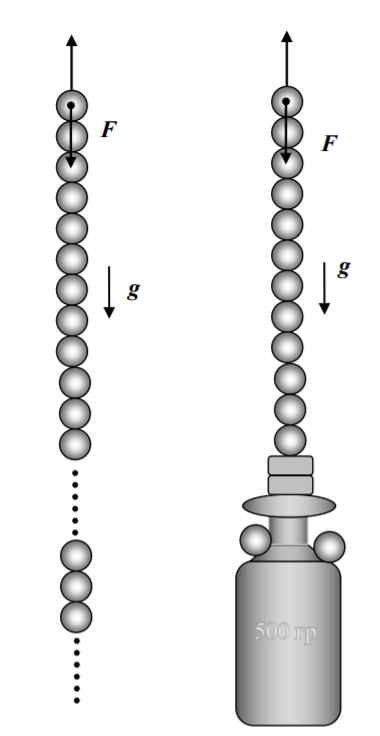
\includegraphics[scale=0.3]{picks/121-scheme1.png} \\
        \textit{Рис. 1. Магнитный момент неод. шариков}

    \end{center}
}
\shiftedText{0.1cm}{4.5cm}
{
    \begin{center}
    
        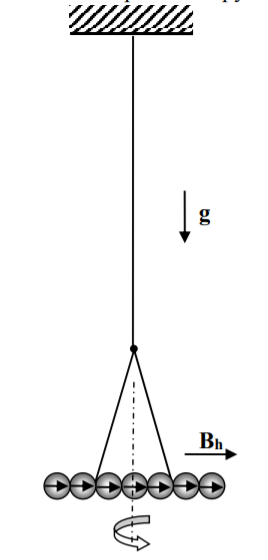
\includegraphics[scale=0.3]{picks/121-scheme2.png} \\
        \textit{Рис. 2. Крутильный маятник}
    
    \end{center}
}
\shiftedText{0.1cm}{6cm}
{
    \begin{center}

        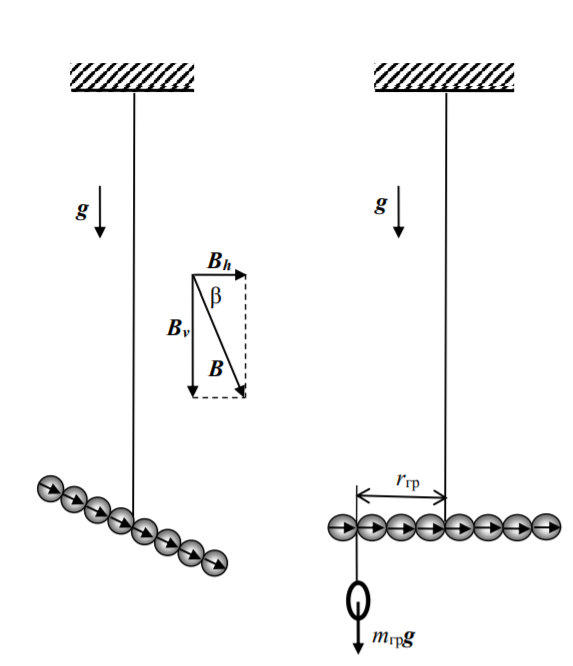
\includegraphics[scale=0.3]{picks/121-scheme3.png} \\
        \textit{Рис. 3. Определение вертикальной составляющей поля земли}

    \end{center}
}
\end{center}

\subsection{Формулы и приближения}

\formula {Магнитный момент витка с током:} {coilMagMomentum}
{
    \vec{P_m} = \frac{I}{c} \cdot \vec{S} = \frac{IS}{c} \cdot \vec{n}
}

\formula {Поле магнитного диполя:}{coilField}
{
    \vec{B} = \frac{3\left( \vec{P_m} \vec{r} \right) \vec{r}} {r^5} - \frac{\vec{P_m}}{r^3}
}

\formula {Механический момент, действующий на диполь в магнитном поле:}{coilForceMomentum}
{
    \vec{M} = \vec{P_m} \times \vec{B}
}

\formula {Сила взаимодействия 2 маленьких магнитов:}{twoMagnForce}
{
    F = \frac{-6P_m^2}{r^4}
}

\subsubsection{Неодиомовые магнитные шары}
В настоящей работе используются неодимовые магниты шарообразной формы.
\noindentДля этих шаров выполняется:

\shiftedText{0.3cm}{14cm}
{
    \begin{enumerate}
        \item Они намагничены однородно.
        \item Вещество, из которого изготовлены магниты, является магнитожёстким материалом.
        \item Поле такого магнита с хорошей точностью можно считать полем точечного магнитного диполя.
    \end{enumerate}
}

\newpage

\formula {Cила сцепления магнитных шариков}{ballsForce}
{
    F_0 = \frac{F}{1,08}
}

\formula {Период колебаний магнитной стрелки}{period}
{
    T(n) = \pi n \sqrt{\frac{md^2}{3P_m B_h}}\,,
}
где \mth{B_h} - горизонтальная составляющая магнитного поля земли. \\[0.5cm]

\formula {Вертикальная составляющая магнитного поля земли:}{verticalForceProjection}
{
    m\ruB{гр} g r\ruB{гр} = P_0 B_\nu = n P_m B_\nu
}